\documentclass[border=10pt]{standalone}
\usepackage{tikz}

\begin{document}
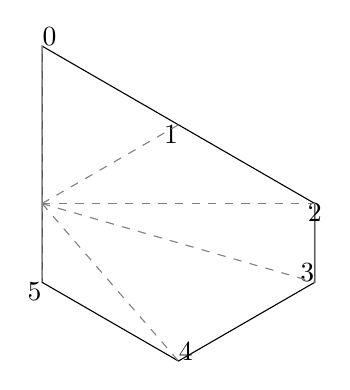
\begin{tikzpicture}[scale=2]
    % Define the coordinates of the hexagon vertices
    \coordinate (A) at (0, 1);
    \coordinate (B) at (0.866, 0.5);
    \coordinate (C) at (1.732, 0);
    \coordinate (D) at (1.732, -0.5);
    \coordinate (E) at (0.866, -1);
    \coordinate (F) at (0, -0.5);

    % Draw the hexagon
    \draw[black] (A) -- (B) -- (C) -- (D) -- (E) -- (F) -- cycle;

    % Label the vertices
    \node[anchor=south west, inner sep=0pt] at (A) {0};
    \node[anchor=north east, inner sep=0pt] at (B) {1};
    \node[anchor=north, inner sep=0pt] at (C) {2};
    \node[anchor=south east, inner sep=0pt] at (D) {3};
    \node[anchor=south west, inner sep=0pt] at (E) {4};
    \node[anchor=north east, inner sep=0pt] at (F) {5};

    % Optional: Draw lines from center to vertices
    \foreach \point in {A,B,C,D,E,F} {
        \draw[dashed, gray] (0,0) -- (\point);
    }
\end{tikzpicture}
\end{document}